\documentclass{report}
\usepackage{graphicx}
\usepackage{csvsimple}
\usepackage[T5]{fontenc}
\usepackage[a4paper, top=2cm, bottom=2cm, left=2cm, right=2cm]{geometry}

\renewcommand{\thesection}{\arabic{section}}

\begin{document}

\begin{titlepage}
    \center
    \LARGE{Vietnam Posts and Telecommunications Institute of Technology (PTIT)} \\
    \vspace*{\fill}
    
    
\includegraphics[scale=0.5]{ptit-logo.png} \\
    \vspace{1cm}
    \huge\textbf{Python 2nd Assignment \\ Image Classification} \\
    \vspace{1cm}

    \Large
    \begin{tabular}{@{}lll@{}}
    Students: & Trần, Vũ Tiến Minh & B23DCCE067 \\
              & Phạm, Quốc Hùng    & B23DCVT188 \\
    Lecturer: & Dr. Kim, Ngọc Bách &            \\
    Class:    & D23CQCE04-B        &            \\
    Date:     & \today             &            \\  
    \end{tabular}

    \vspace{\fill}
\end{titlepage}

\chapter*{Introduction}
This report is the justification and results for the assignment. The assignment focuses on building, training and 
testing two simple neural networks to classify the CIFAR-10 dataset: A three layers Multi-Layer Perceptron 
(MLP) and a three convolution layers Convolutional Neural Network (CNN).

\section*{The Assignment Tasks}
These are the main tasks:
\begin{itemize}
    \item Build a basic MLP (Multi-Layer Perceptron) neural network with 3 layers.
    \item Build a Convolutional Neural Network (CNN) with 3 convolution layers.
    \item Perform image classification using both neural networks, including training, validation, and testing.
    \item Plot learning curves.
    \item Plot confusion matrix.
    \item Use the PyTorch library.
\end{itemize}

\section*{Packages Dependencies}
These packages are centered around working with the PyTorch library as the requirement has stated:
\begin{itemize}
    \item \texttt{torch}: For building and training neural networks.
    \item \texttt{torchvision}: For getting datasets and image transformations.
    \item \texttt{scikit-learn}: For train/validation splitting and calculating confusion matrix.
    \item \texttt{numpy}: For numerical operations.
    \item \texttt{matplotlib}: For plotting learning curves, confusion matrices and others.
\end{itemize}

\newpage
\tableofcontents
\newpage

\chapter*{Report}

\section{CIFAR-10 Dataset}
CIFAR-10 dataset is a well-known dataset for image classification exercise. It has 60,000, $32\times32$ pixels images 
in 10 classes, with 6,000 images per class. PyTorch library splits the dataset into 50,000 training images and 
10,000 testing images. 

\begin{figure}[ht]
    \center
    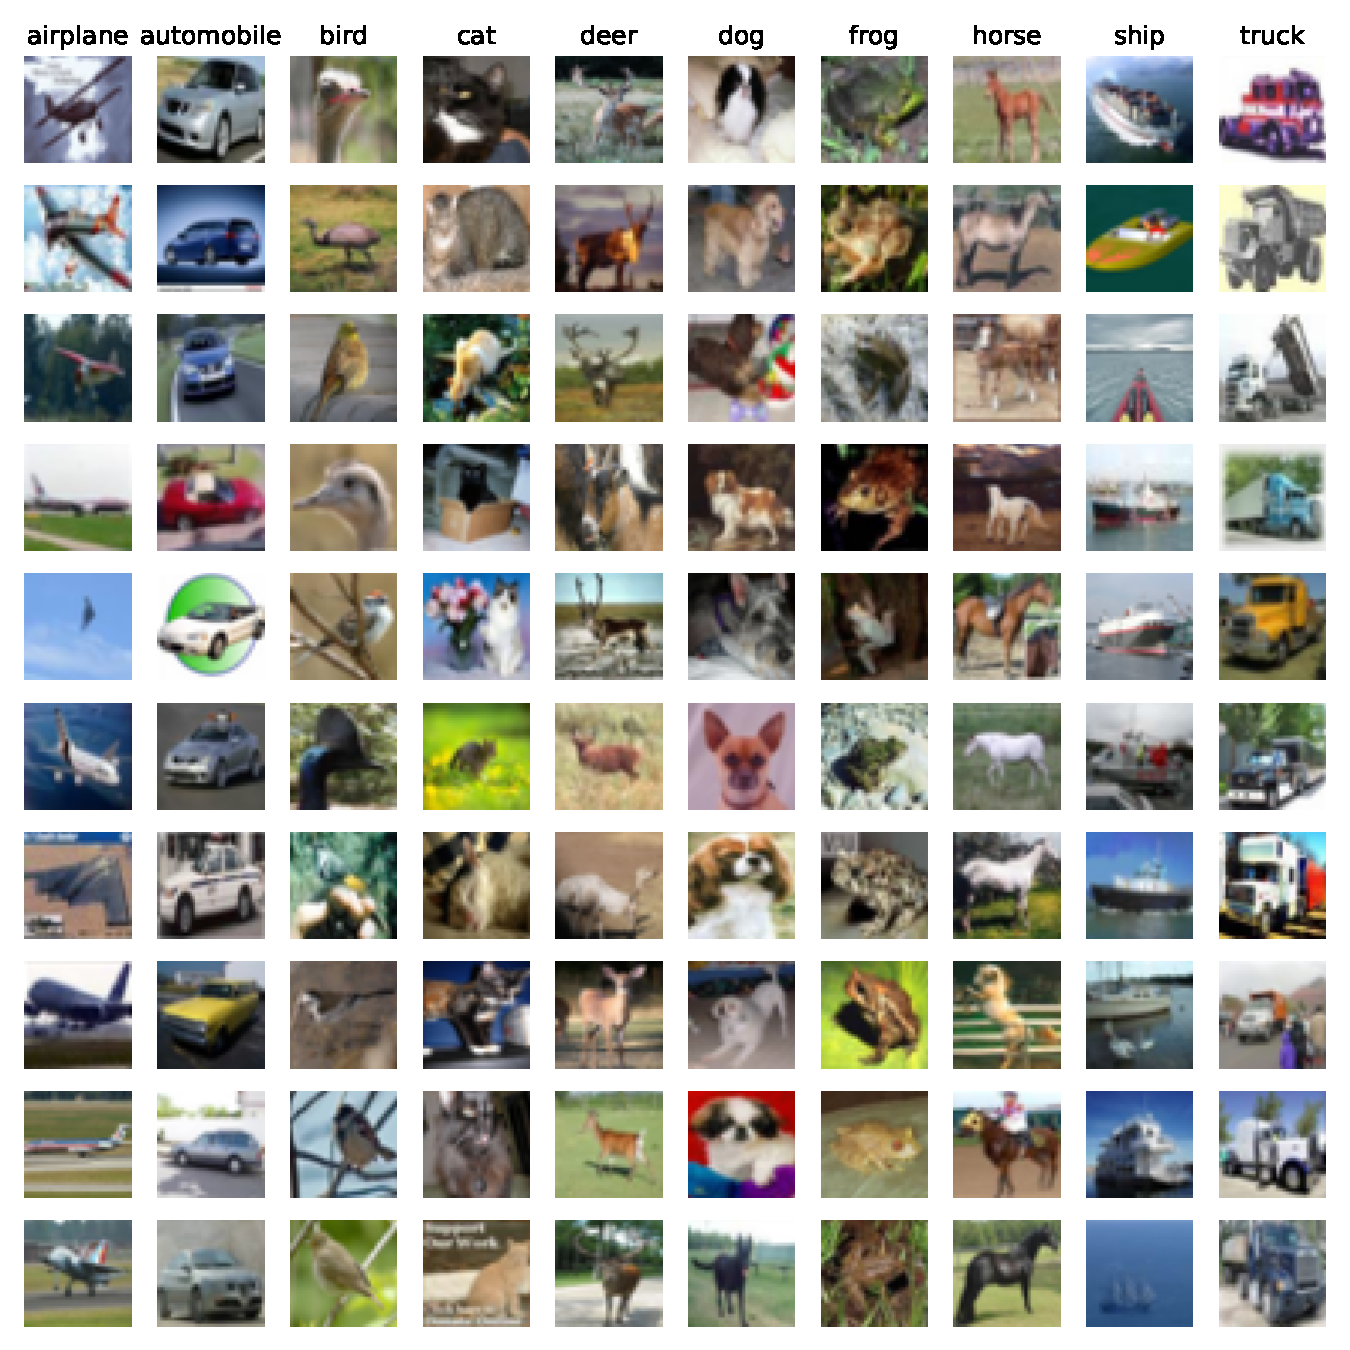
\includegraphics[scale=0.7]{../output/cifar10-images.pdf}
    \caption{cifar10-images.pdf}
\end{figure}

In this project, to do training validation and testing seperately, the 50.000 images set is split into 40,000 
training images and 10,000 validation images. This is a common method tune the model based on the validation 
set's results, and then testing the model with the test set to have an unbiased evaluation of the model.

\section{Data Analysis}
The first step of any Machine Learning exercise is to do Data Analysis. All analysis will be done on the 40,000 
images train set only. This is to simulate the real world scenario, where the test set is not available during the 
training process. The validation set is used for tuning the model, so it is not used in the analysis.

\subsection{Color Distribution} 
The below graph shows the RGB color distribution of the dataset, with the color intensity ranging from 0 to 
255. Based on the graph, all three channels does follow a Gaussian distribution to some degree, minus the very 
high peak at the 255 region. The blue channel specifically is right skewed, so unlike other distribution with a 
mean around 128, blue has a mean around 100.

\begin{figure}[ht]
    \center
    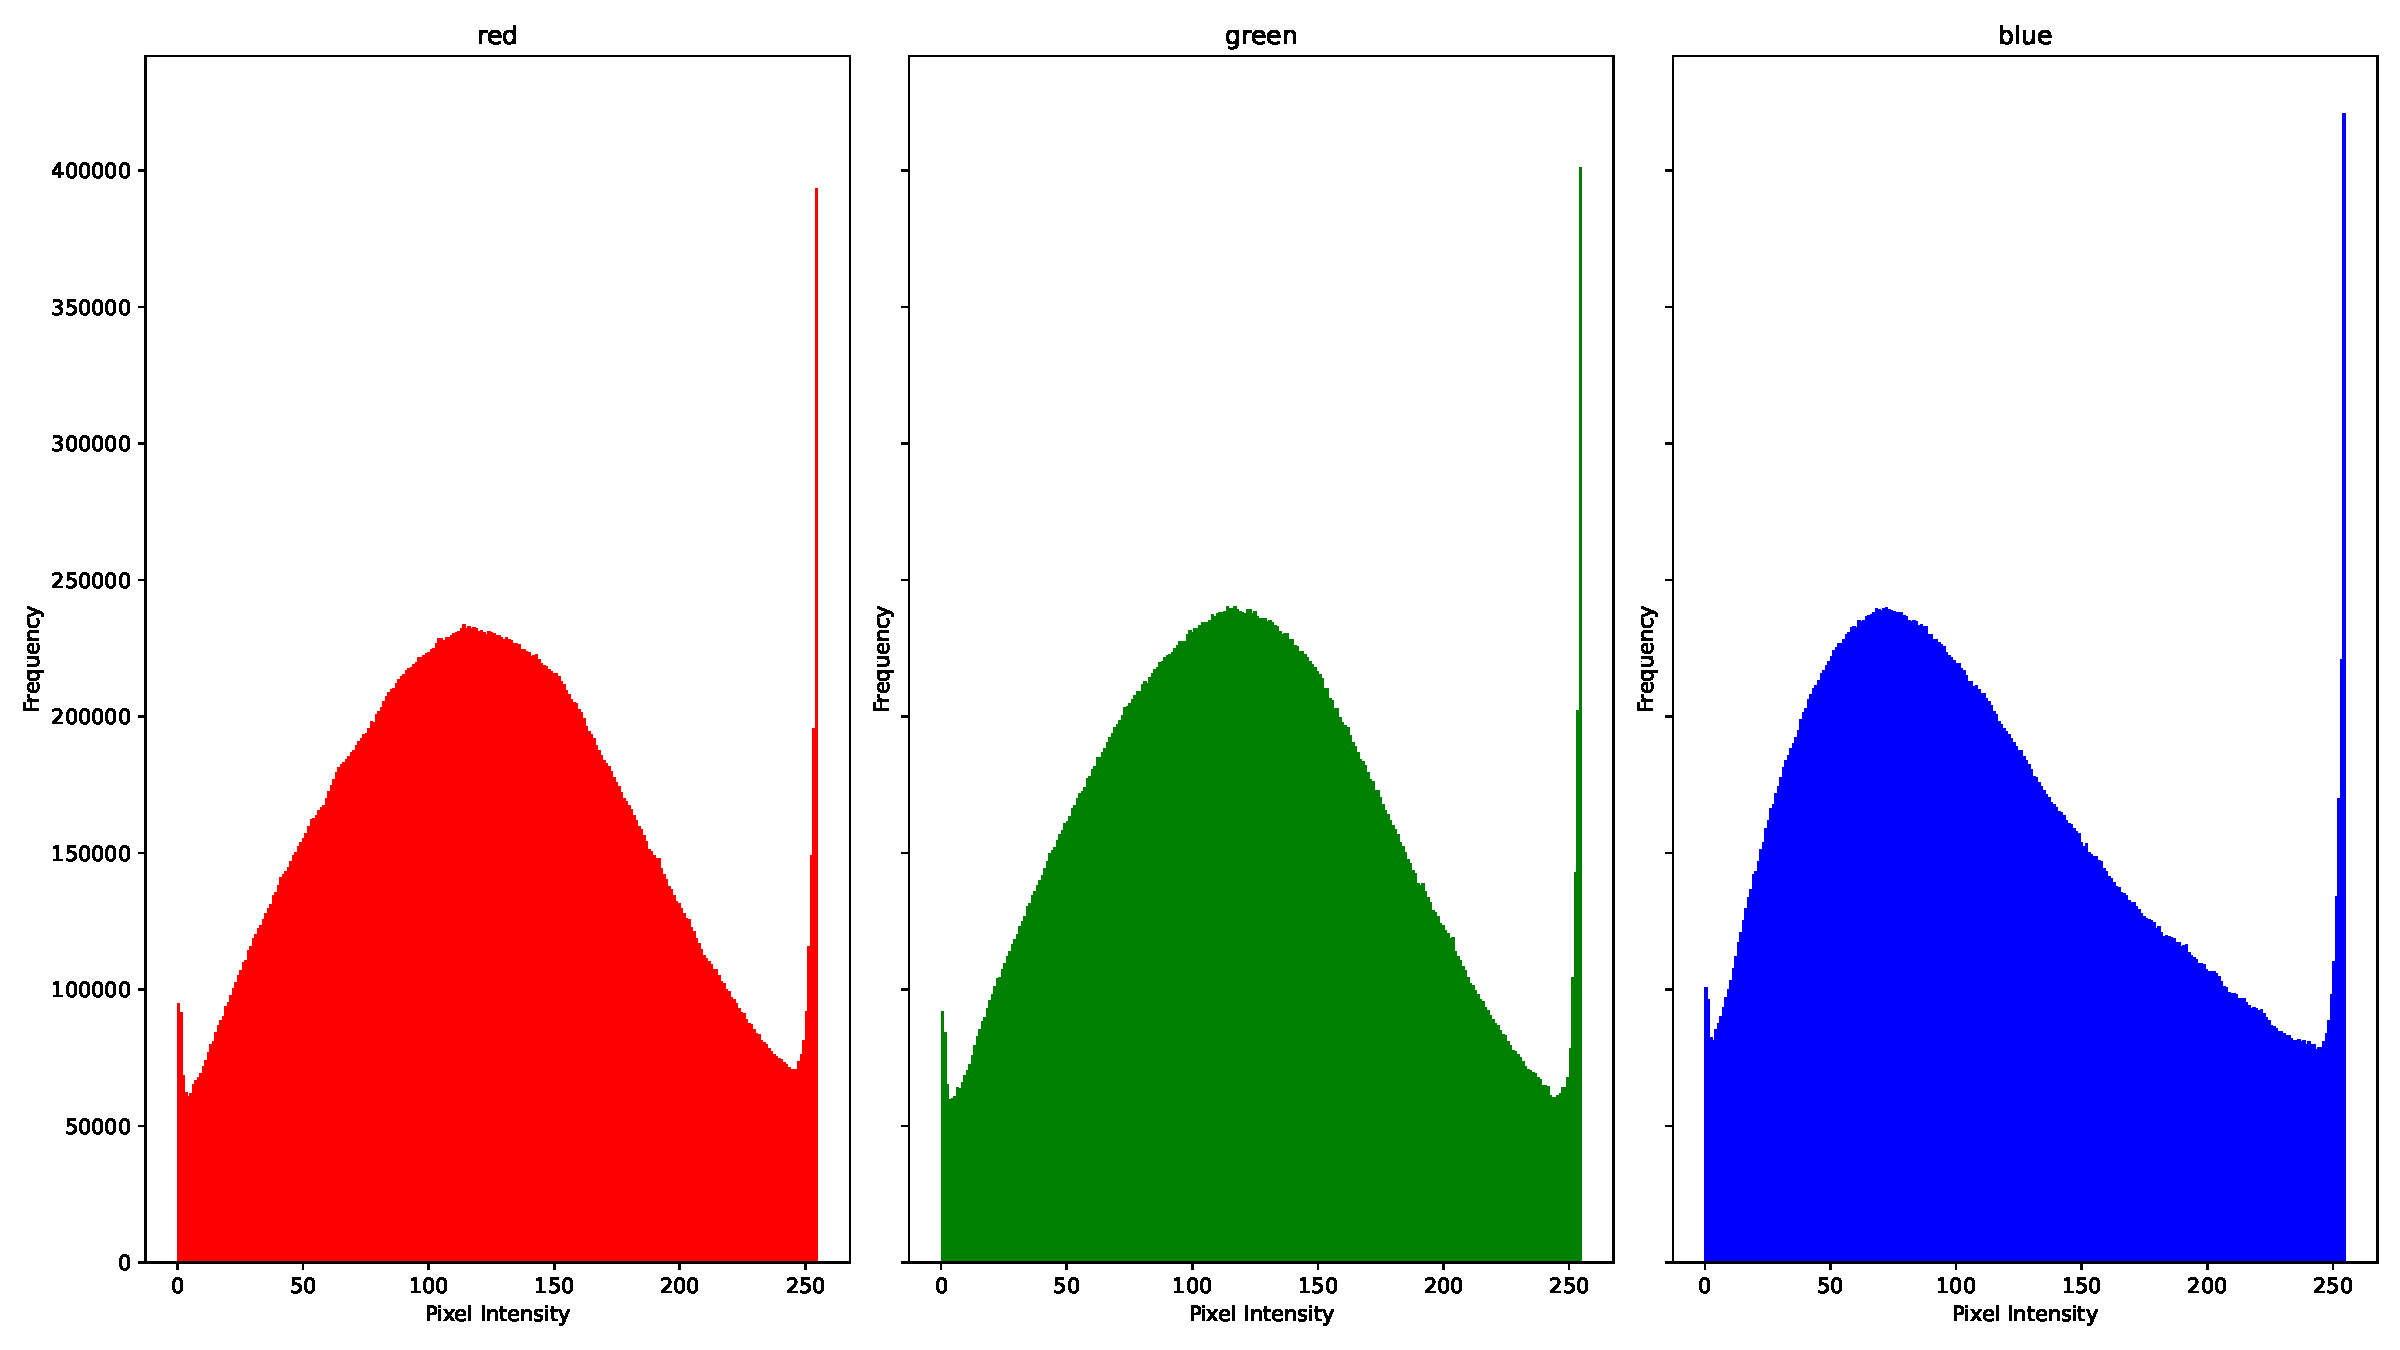
\includegraphics[scale=0.4]{../output/cifar10-channels.pdf}
    \caption{cifar10-channels.pdf}
\end{figure}

\subsection{Mean And Standard Deviation} 
MLP and CNN can perform better on a normalized dataset, often resulting in a faster convergence and better 
accuracy. In PyTorch, \texttt{torchvision.transforms.Normalize} function normalizes images by adjusting their 
pixel values according to the mean and standard deviation of the dataset. So the next step is to find the mean 
and standard deviation. The table includes the raw values and also the normalized values divided by 255.

\begin{table}[ht]
    \center
    \csvautotabular{../output/cifar10-mean-std.csv}
    \caption{cifar10-mean-std.csv}
\end{table}

\subsection{Transform Dataset}
Finally, all three datasets are transformed.\texttt{torchvision.transforms.ToTensor()} converts each image from 
shape of $32\times32\times3$ to a tensor with shape of $3\times32\times32$.

\newpage
\begin{verbatim}
    # python
    from torchvision import transforms

    transform = transforms.Compose([
        transforms.ToTensor(),
        transforms.Normalize(mean, std)
    ])
\end{verbatim}

\section{Building Models}
To keep the program simple, both models' hyper parameters are tuned by hand after each training/validation 
cycle until the performance is deemed high enough. Below are the structure of the two models.

\subsection{Multi-Layer Perceptron}
The MLP model used for this assignment consists of three fully connected linear layers:

\begin{verbatim}
    # python
    from torch import nn

    relu = nn.ReLU()
    dropout = nn.Dropout(0.2)
    
    model = nn.Sequential(                  # (_, 3, 32, 32)
        nn.Flatten(),                       # (_, 3 * 32 * 32)

        nn.Linear(3 * 32 * 32, 512),        # (_, 512)
        nn.BatchNorm1d(512),
        relu,
        dropout,

        nn.Linear(512, 256),                # (_, 256)
        nn.BatchNorm1d(256),
        relu,
        dropout,

        nn.Linear(256, 10)                  # (_, 10)
    )
\end{verbatim}

\begin{enumerate}
    \item \textbf{Flatten Layer:} Converts the input image into a 1D vector.
    \item \textbf{First Linear Block:}
    \begin{itemize}
        \item Fully connected layer with 512 output units.
        \item Batch normalization for improved training stability.
        \item ReLU activation for non-linearity.
        \item Dropout 20\% for regularization.
    \end{itemize}
    \item \textbf{Second Linear Block:}
    \begin{itemize}
        \item Fully connected layer with 256 output units.
        \item Batch normalization.
        \item ReLU activation.
        \item Dropout 20\%.
    \end{itemize}
    \item \textbf{Output Linear Layer:} Fully connected layer mapping to 10 output classes.
\end{enumerate}

\subsection{Convolutional Neural Network}
The CNN model used for this assignment consists of three convolution layers and one output linear layer:

\begin{verbatim}
    # python
    from torch import nn

    relu = nn.ReLU()
    maxpool = nn.MaxPool2d(2, stride=2)
    dropout = nn.Dropout2d(0.2)

    model = nn.Sequential(                  # (_, 3, 32, 32)
        nn.Conv2d(3, 128, 3, padding=1),    # (_, 128, 32, 32)
        nn.BatchNorm2d(128),
        relu,
        maxpool,                            # (_, 128, 16, 16)
        dropout,

        nn.Conv2d(128, 256, 3, padding=1),  # (_, 256, 16, 16)
        nn.BatchNorm2d(256),
        relu,
        maxpool,                            # (_, 256, 8, 8)
        dropout,

        nn.Conv2d(256, 512, 3, padding=1),  # (_, 512, 8, 8)
        nn.BatchNorm2d(512),
        relu,
        maxpool,                            # (_, 512, 4, 4)
        dropout,

        nn.Flatten(),                       # (_, 512 * 4 * 4)
        nn.Linear(512 * 4 * 4, 10)          # (_, 10)
    )
\end{verbatim}

\begin{enumerate}
    \item \textbf{First Convolutional Block:}
    \begin{itemize}
        \item 2D convolution: 3 input channels, 128 output channels, $3\times3$ kernel, padding=1. The padding=1 is 
              for preserving the dimensions from $30\times30$ to $32\times32$.
        \item Batch normalization.
        \item ReLU activation.
        \item $2\times2$ Max pooling reduces size to $16\times16$.
        \item Dropout 20\%.
    \end{itemize}
    \item \textbf{Second Convolutional Block:}
    \begin{itemize}
        \item 2D convolution: 128 input to 256 output channels.
        \item Batch normalization.
        \item ReLU activation.
        \item $2\times2$ Max pooling for size of $8\times8$.
        \item Dropout 20\%.
    \end{itemize}
    \item \textbf{Third Convolutional Block:}
    \begin{itemize}
        \item 2D convolution: 256 input to 512 output channels.
        \item Batch normalization.
        \item ReLU activation.
        \item $2\times2$ Max pooling for size of $4\times4$.
        \item Dropout 20\%.
    \end{itemize}
    \item \textbf{Output Linear Layer:}
    \begin{itemize}
        \item Flatten layer converts feature maps to a vector size of $512\times4\times4$.
        \item Fully connected linear layer mapping to 10 output classes.
    \end{itemize}
\end{enumerate}

\section{Optimizers And Criterions}
Now comes the most important part of the exercise: Optimize the optimizers. Similar to building the models, 
the below optimizers and parameters were manually tuned after each validation results.

\subsection{}

\begin{itemize}
    \item \textbf{Optimizer:} Both models use the \texttt{torch.optim.Adam} optimizer. Adam is chosen for its adaptive learning rate and generally faster convergence compared to SGD, especially for deep networks.
    \item \textbf{Learning Rate:} The initial learning rate is set to $0.001$. This value provided a good balance between convergence speed and stability. Higher values led to divergence, while lower values slowed down training.
    \item \textbf{Weight Decay:} A weight decay (L2 regularization) of $1 \times 10^{-4}$ is used to help prevent overfitting.
    \item \textbf{Other Parameters:} Default values for $\beta_1=0.9$ and $\beta_2=0.999$ are used, as they work well in most cases.
\end{itemize}

\textbf{Loss Function:} Both models use \texttt{torch.nn.CrossEntropyLoss}, which is standard for multi-class classification problems. It combines \texttt{LogSoftmax} and \texttt{NLLLoss} in one single class, making it suitable for the 10-class CIFAR-10 dataset.

\begin{verbatim}
    # python
    from torch import nn, optim

    optimizer = optim.Adam(model.parameters(), lr=0.001, weight_decay=1e-4)
    criterion = nn.CrossEntropyLoss()
\end{verbatim}

These choices were validated by monitoring the learning curves and validation accuracy. If the model overfit or failed to converge, learning rate and weight decay were adjusted accordingly.
 


% And Loss Function: Explain the choosen loss function and optimizers' parameters.
%     \item Training and Validation: Justify the implemented methods.
%     \item The Results: Discuss the learning curve and confusion matrix.
% \end{itemize}


% I just want to be cold

\end{document}